\documentclass[margin=5mm]{standalone}
\usepackage[dvipsnames]{xcolor}
\usepackage{pgfplots}
\usepackage{tikz}

\pgfplotsset{compat=1.18}
\begin{document}

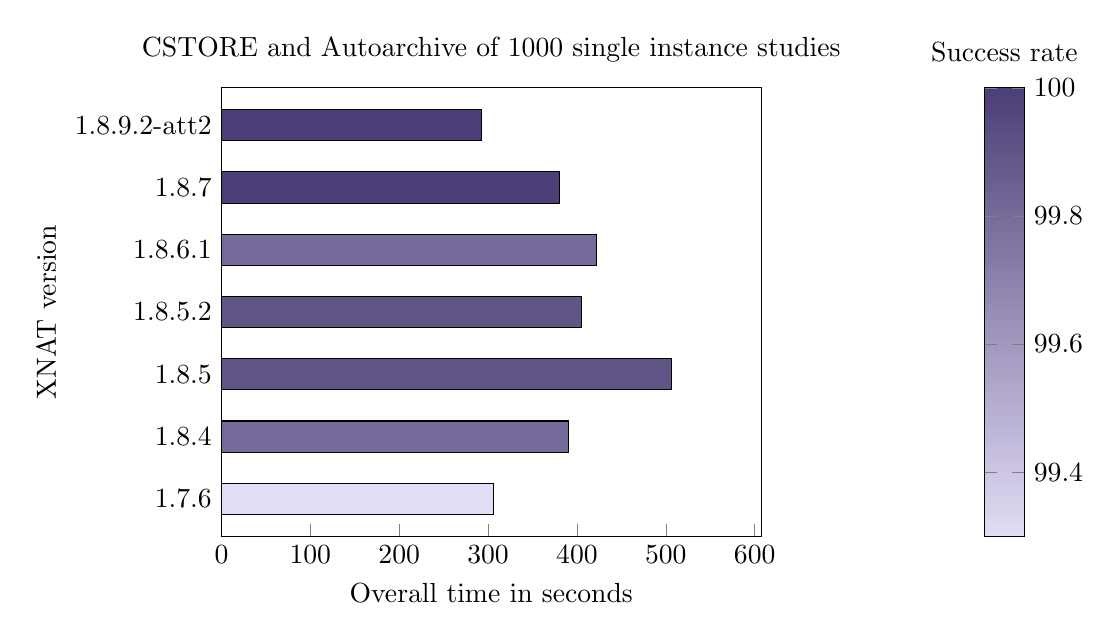
\begin{tikzpicture}
    \begin{axis}[
        align = center,
        xlabel = Overall time in seconds,
        ylabel = XNAT version,
        xtick pos = left,
        ytick pos = left,
        ytick = data,
        xmin = 0,
        enlarge x limits = {value = 0.2, upper}, % make node labels not overlap with axes
        title = {CSTORE and Autoarchive of 1000 single instance studies},
        title style = {text width = 0.8\textwidth},
        yticklabels = {1.7.6,1.8.4,1.8.5,1.8.5.2,1.8.6.1,1.8.7,1.8.9.2-att2},
        colorbar,
        colorbar style = {xshift = 1cm, title = Success rate},
        colormap={successcolormap}{rgb255(0)=(226, 220, 245) rgb255(1000)=(76, 62, 118)},
        scatter,
        scatter src = x,
        only marks,
        visualization depends on={\thisrow{x} \as \barlength},
        scatter/@pre marker code/.append code={,
            \fill [draw=black] (axis direction cs:0,0.25) rectangle (axis direction cs:{-1 * \barlength},-0.25);,
            \pgfplotsset{mark = none},
        },
        point meta=\thisrow{successrate}
    ]
        \addplot table[x = x,y expr=\coordindex] {
            x    y    successrate
            305.7 1.7.6 99.3
            390.3 1.8.4 99.8
            506.0 1.8.5 99.9
            404.8 1.8.5.2 99.9
            421.8 1.8.6.1 99.8
            380.6 1.8.7 100.0
            292.3 1.8.9.2-att2 100.0
        };
    \end{axis}
\end{tikzpicture}

\end{document}